\documentclass[9pt,a4paper]{article}

\usepackage{fullpage}
\usepackage{parskip}
\usepackage{authblk}
\usepackage{tikz}
\usepackage{graphicx}
\usepackage{caption}
\usepackage{tikz}
\usepackage[margin=2.5cm]{geometry}
\usepackage{titlesec}
\usetikzlibrary{circuits.ee.IEC,circuits.logic.US}
\usepackage[european,smartlabels]{circuitikz}


\begin{document}

\title{ARM Report}
\author{Ziming Feng}
\author{Zhan Shi}
\author{Zihao Zhao}
\author{Xinhe Wang}
\affil{Group 38}

\date{}

\maketitle
\vspace{-2em}

% Grabbed from https://www.overleaf.com/learn/latex/LaTeX_Graphics_using_TikZ%3A_A_Tutorial_for_Beginners_(Part_3)%E2%80%94Creating_Flowcharts
\usetikzlibrary{shapes.geometric, arrows}
% TikZ flowchart styles
\tikzstyle{startstop} = [rectangle, rounded corners, minimum width=3cm, minimum height=1cm, text centered, draw=black, fill=red!30]
\tikzstyle{io} = [trapezium, trapezium left angle=70, trapezium right angle=110, minimum width=3cm, minimum height=1cm, text centered, draw=black, fill=blue!30]
\tikzstyle{process} = [rectangle, minimum width=3cm, minimum height=1cm, text centered, text width=4cm, draw=black, fill=orange!30]
\tikzstyle{decision} = [diamond, minimum width=3cm, minimum height=1cm, text centered, draw=black, fill=green!30]
\tikzstyle{arrow} = [thick,->,>=stealth]

\section{Assembler}

\noindent
\begin{minipage}[t]{0.52\textwidth}
\vspace{0pt}
Our implementation of the assembler consists of several modules and follows what the spec suggested.

\vspace{\baselineskip}
First of all, the table module defines the symbol table, which maps labels to their corresponding addresses. We defined the \verb|Entry| struct in a linked list style, where each node stores a key-value pair and a pointer to the next node. The \verb|Table| struct comprises a \verb|head| and a \verb|tail| pointer, referencing the first and last entries in the table, respectively.

\vspace{\baselineskip}
In addition, the \verb|pass| module performs two passes over the source code. The first pass builds a symbol table to store the label-address pairs, while the second pass is used to generate the corresponding binary representations and write them to the output file.

\vspace{\baselineskip}
The \verb|tokenizer| module includes a single function that breaks down an assembly instruction into individual tokens. These tokens are then processed by a large, single function defined in the parser module, which converts them into an intermediate representation defined in the \verb|intermediate_reps.h| file.

\vspace{\baselineskip}
To generate the final binary instructions, we use the \verb|assemble_instructions| module, which translates the intermediate representation of an assembly instruction into its binary form. Within this module, the \verb|assemble_instructions| function utilises four static helper functions, each dedicated to handling a specific type of instruction, except for the \verb|assemble_load_store| function which is designed to handle both single data transfer and load literal instructions.

\vspace{\baselineskip}
Finally, the \verb|assemble.c| file includes a static helper function to assemble the instructions from the source file into the output file, and the \verb|main| function to serve as the entry point of the assembler program.
\end{minipage}
\hfill
\begin{minipage}[t]{0.45\textwidth}
\vspace{0pt}
\centering
\scalebox{0.5}{
      \begin{tikzpicture}[node distance=2.65cm]
        % Nodes
        \node (start) [startstop] {Start};
        \node (init_table) [process, below of=start] {Initialise symbol table};
        \node (open_file) [process, below of=init_table] {Open source file and output file};
        \node (pass1) [process, below of=open_file] {First pass};
        \node (eof1) [decision, below of=pass1, yshift=-0.25cm] {File-in EOF?};
        \node (entry) [process, below of=eof1] {Put label-address entry into symbol table};
        \node (pass2) [process, below of=entry, xshift=4cm, yshift=-0.25cm] {Second pass};
        \node (eof2) [decision, below of=pass2] {File-in EOF?};
        \node (parse) [process, below of=eof2] {Tokenising and parsing};
        \node (ass_instr) [process, below of=parse] {Assemble intermediate representation};
        \node (write) [process, below of=ass_instr] {Write binary instruction into output file};
        \node (close) [process, below of=write, xshift=3cm, yshift=-0.25cm] {Close source file and output file};
        \node (stop) [startstop, below of=close] {Stop};


        % Arrows
        \draw [arrow] (start) -- (init_table);
        \draw [arrow] (init_table) -- (open_file);
        \draw [arrow] (open_file) -- (pass1);
        \draw [arrow] (pass1) -- (eof1);
        \draw [arrow] (eof1) -- node[anchor=east] {no} (entry);
        \draw [arrow] (entry) -- ++(-3cm,0) |- (eof1);
        \draw [arrow] (eof1) -| node[anchor=south east, xshift=-1cm] {yes} (pass2);
        \draw [arrow] (pass2) -- (eof2);
        \draw [arrow] (eof2) -- node[anchor=east] {no} (parse);
        \draw [arrow] (parse) -- (ass_instr);
        \draw [arrow] (ass_instr) -- (write);
        \draw [arrow] (write) -- ++(-3cm,0) |- (eof2);
        \draw [arrow] (eof2) -| node[anchor=south east, xshift=-0.5cm] {yes} (close);
        \draw [arrow] (close) -- (stop);

      \end{tikzpicture}
}

\captionof{figure}{Procedure of the assembler}
\end{minipage}

\newpage
\section{Part III}

To implement the blinking LED on the Raspberry Pi 3B, we proceeded through the structured steps suggested by the spec.

Hardware-wise, we connected GPIO pin 9, a random GPIO pin we chose, to the anode of an LED on a breadboard via a 220$\Omega$ resistor, and the cathode to ground using two M2F wires.

To light up the LED, we produced an AArch64 assembly program under the subset given in previous parts, making it compatible with our assembler built in part 2.
In the assembly, we first put the value \verb|0x3f200000| into register \verb|w0| using the \verb|movz| instruction with left shift as the base pointer to RPi memory, preparing to modify GPIO settings and signal via RPi registers later on.
Subsequently, the value \verb|0x08000000| is put into register \verb|w1| using \verb|movz| and written to the GPFSEL0 register on RPi using the \verb|str| instruction and address stored in \verb|w0|. This should successfully set GPIO pin 9 to output mode.
Then, the values \verb|0x3f20001c| and \verb|0x3f200028| are loaded into \verb|w0| and \verb|w1| respectively, using the \verb|add| instruction to represent the memory address of GPSET0 and GPCLR0 registers for later modification.

After that, we created a label called \verb|loop|, grouping the instructions to be executed in an infinite loop.
Inside the loop, the value \verb|0x0200| is written to the addresses in \verb|w0| and \verb|w1| in an alternating way using the \verb|str| instruction to make the GPIO pin send a high or low signal.
The instructions to send high signals are under the label loop, while the instructions to send low signals are under another label called \verb|turn_off|, so that we can branch to different locations after the delay.

Between sending alternating signals, we added a constant delay to make the LED blinking visible to the human eye.
The delay was implemented using the basic repeated decrement approach, and the related instructions were grouped under two different labels.
These two delay labels both comprise decrementing register \verb|x3|, which was set with a value beforehand using the \verb|subs| instruction, followed by the \verb|b.ne| instruction to finish the loop.
The only difference between the two labels is that one branches to sending high signals and the other branches to sending low signals, simulating the two stretches of delay.

Originally, we intended to use the \verb|br| instruction with the label address stored in a register to use only one delay loop.
However, our assembler does not feature storing the address of a label directly, only the content at the address of the label.
Therefore we had to resort to using two different delay loops with duplicate instructions.

  \begin{center}
    \begin{circuitikz}
        \draw (0,0) node[left]{GPIO 9} to[european resistor,l=220$\Omega$] (2,0) to[led] (4,0) -- (4,0) node[right]{GND} node[ground]{};
      \end{circuitikz}
    \captionof{figure}{LED circuit diagram}
  \end{center}

\section{Extension}

For the extension, we completed two tasks: comment support for the assembler and a counter based on a Raspberry Pi bare metal.

\subsection{Comment support for assembler}

Following the suggestions in the spec, we decided to extend our assembler to allow the C-style line and block comments in .s files.

We implemented a static helper function, \verb|remove_comments|, to strip both single-line and block comments from a given line of assembly code.
It extracts the uncommented part of the line of code into a buffer, allowing the pass phase to process it as if there were no comments in the line.
This function takes two parameters: a string line and a pointer to a boolean value indicating whether the string line is currently within a block comment. If the line contains a single-line comment, we ignore the characters from the single-line comment marker up to the end of the line. If the string line is within a block comment, we ignore the content within the block comment boundaries.
This helper function is able to parse the comments without removing the original comments from the source file.

Initially, our approach for supporting C-style comments in assembly files was to extract the uncommented portions of each line to an intermediate file during the parsing phase.
We then intended to assemble the instructions from this intermediate file. However, this method failed in some test cases from both the test suite and the additional test cases we created, resulting in an error indicating that the intermediate file could not be opened.
Despite validating our code logic, we continued to experience errors when opening files. The technique was also laborious, requiring us to copy uncommented segments into another file.
Consequently, we chose to discontinue this approach and instead parse each line during the two-pass phase.

To rigorously test this, we wrote a shell script to generate assembly files with randomly injected comments and compared the output \verb|.bin| files with their clean counterparts.
This stress test brought our test case count to approximately 1200, ensuring a high level of reliability.

\subsection{Raspberry Pi based counter}

\subsubsection{Design}

The counter consists of a seven-segment display that either counts upwards from 0 to 9 or downwards from 9 to 0, a button which changes the counting direction at any moment, and a separate button to act as a switch for the counter.
The display is mounted on a breadboard with its common cathode connected to the 3.3V pin on the Raspberry Pi.
The other 7 pins that control individual segments are wired to different GPIO pins respectively.
Under this layout, a segment lights up when the corresponding GPIO pin is cleared, creating a potential difference, and dims when the pin is set.
We wired the buttons from separate GPIO pins to a ground pin, both parallel to the display.
The control of the counter generally follows the same idea as part 3, but is achieved using C instead of assembly programs.
This is the reason of using bare metal instead of an OS on the RPi.

In terms of detail, mode selection of the GPIO pins is implemented via a separate \verb|config.txt| file which sets specific GPIO pins at boot time, and it is loaded into the RPi alongside the \verb|kernal8.img| file.
The seven pins connected to individual segments are set to \verb|op| for output, and the button pins are set to \verb|pu| to enable an internal pull-up resistor.
Consequently, when a button is not pressed (open circuit), the resistor completes an internal circuit from 3.3V to the pin and the pin has a defined state of 1.
When the button is pressed (closed circuit), the current flows through the complete circuit of 3.3V to ground via the button. Hence the pin would have 0V, which represents digital state 0.
The display logic and register manipulation are implemented in the \verb|main.c| file, which would then be cross-compiled into \verb|kernel8.img|.
Inside \verb|main.c|, register manipulation of the RPi is achieved via pointers to the respective addresses and is grouped into more intuitive macros.
Ultimately, corresponding pins are set and cleared to show different numbers on the display.
A precise delay between consecutive numbers is added via the system timer of the Raspberry Pi, which runs at 1 MHz on bare metal, allowing time-specific delay as opposed to simple decrement loops.

Finally, the state of a button is determined by inspecting the GPLEV register of the RPi, which records the digital state of the specific pin.
The pin would have a digital state of 1 when the button is not pressed, and 0 when the button is pressed.
Whenever the button controlling the counting direction is pressed and released, a static global flag is negated, taking effect immediately.
Furthermore, when the switch is off the counter turns blank, and when the switch is back on the counter resumes from the last digit.
The \verb|check_button| and \verb|check_switch| functions are called each iteration inside the delay function to maximise the time for detection.

\noindent
\begin{minipage}[t]{0.4\textwidth}
\centering
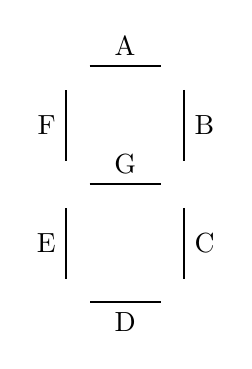
\begin{tikzpicture}[scale=1.5]
    % Seven segment display
    \draw[thick] (0.2,2) -- (0.8,2) node[midway,above] {A};

    \draw[thick] (1,1.8) -- (1,1.2) node[midway,right] {B};

    \draw[thick] (1,0.8) -- (1,0.2) node[midway,right] {C};

    \draw[thick] (0.8,0) -- (0.2,0) node[midway,below] {D};

    \draw[thick] (0,0.2) -- (0,0.8) node[midway,left] {E};

    \draw[thick] (0,1.2) -- (0,1.8) node[midway,left] {F};

    \draw[thick] (0.2,1) -- (0.8,1) node[midway,above] {G};
\end{tikzpicture}
\captionof{figure}{Seven-segment display layout}
\end{minipage}
\hfill
\begin{minipage}[t]{0.6\textwidth}
\centering
\begin{circuitikz}[scale=0.9]
    % 3.3V and resistor at top with horizontal turn
    \draw (4.5,4) -- (4.5,4.5) -- (5,4.5) to[european resistor,l=440$\Omega$] (8,4.5) node[right]{3.3V};

    % Seven segment display representation
    \draw (1,4) rectangle (8,3.5);
    \draw (4.5,3.75) node {Seven-segment display};
    \foreach \x/\label in {1.5/A, 2.5/B, 3.5/C, 4.5/D, 5.5/E, 6.5/F, 7.5/G} {
        \draw (\x,3.5) -- (\x,3.0);
        \draw (\x,3.0) to[led, l_=, bipoles/length=0.8cm] (\x,2.6);
        \draw (\x,2.6) -- (\x,2.2);
    }

    \draw (1.1,2.7) node {A};
    \draw (2.1,2.7) node {B};
    \draw (3.1,2.7) node {C};
    \draw (4.1,2.7) node {D};
    \draw (5.1,2.7) node {E};
    \draw (6.1,2.7) node {F};
    \draw (7.1,2.7) node {G};

    % GPIO label and pin numbers
    \draw (0.5,2.25) node[below] {\textbf{GPIO:}};
    \draw (1.5,2.25) node[below] {24};
    \draw (2.5,2.25) node[below] {25};
    \draw (3.5,2.25) node[below] {27};
    \draw (4.5,2.25) node[below] {17};
    \draw (5.5,2.25) node[below] {13};
    \draw (6.5,2.25) node[below] {23};
    \draw (7.5,2.25) node[below] {18};

    % Button connections
    \draw (4,0.75) node[left]{GPIO 26} to[push button,l=button] (6,0.75) node[right]{GND};
    \draw (4,0.25) node[left]{GPIO 21} to[push button] (6,0.25) node[right]{GND};
\end{circuitikz}
\captionof{figure}{Counter wiring diagram}
\end{minipage}

\subsubsection{Challenges}

The biggest challenge for the counter lies with the direction-control button.
Before transforming our conception into a valid circuit, we first had to read the references to understand the internal pull-up setting for Raspberry Pi, since this was not included in part 3.

The wiring of the display from the RPi was one of the challenges. The display is a common-cathode type—two pins are tied to the cathodes, and all segment pins operate as anodes.
Originally, we attempted to light up the segments by connecting the common cathode to GND and other pins to GPIO pins to send high signals.
However, this layout did not work since the segments, which are individual diodes, only conduct in one direction.
This means that we could only connect the common cathode to a 3.3V output, and the segments to GPIO pins.
Initially, this setup was quite puzzling, but we eventually realised that we could make the GPIO pins send low signals to light up the segments and send high signals to dim them.

Nonetheless, the most difficult part of the button is the logic for press detection. In our aim, the reverse signal should be sent at the release of the button, and it should be able to register the release signal after being held for an arbitrary long time.
However, since checking for the button signal can only be done in a separate function call, we had to resort to a static local variable to record and update the last state of the button, which is compared to the current button state to check for state changes.
A change from the digital state of 0 to 1 would then indicate the release and direction change follows, and no action should be taken for a change from 1 to 0.
The last state is then updated so that the next \verb|check_button| call responds correctly to a button being pressed down. To improve button reliability, we implemented debouncing by storing the timestamp of the last press in a static variable.
When a change in state is detected, the counting direction is only reversed if 50ms has passed since the last reverse.
The \verb|check_switch| function was written similarly.

Another challenge was bare-metal programming on the Raspberry Pi. Standard C runtime and libraries are not available in this environment, compiler generated ELF files cannot be executed directly.

Three files, required for the bare-metal program to run, are placed in the FAT32 partition of the SD card: \verb|bincode.bin|, \verb|start.elf| and \verb|kernel8.img|. \verb|kernel8.img| is the binary generated by the cross-compiler, which contains only the machine code of the program, without ELF headers. Although \verb|start.elf| is in ELF format, \verb|kernel8.img| cannot contain ELF headers, as \verb|start.elf| is executed by the GPU while \verb|kernel8.img| is copied to memory starting at \verb|0x80000|, directly executed by the CPU.  As a result, we had to use \verb|objcopy| to extract the machine code from the ELF file generated by the cross-compiler, and write it to \verb|kernel8.img|, which is then loaded into memory by the GPU on Raspberry Pi.

We mainly encountered three challenges in bare-metal programming on the Raspberry Pi:

\begin{enumerate}

  \item The entry point of the program is not necessarily the \verb|main| function, but the first instruction in \verb|kernel8.img|. There's no guarantee that the \verb|main| function in C code is at the beginning of the binary file, so we had to write a \verb|boot.S| file to define the \verb|.text.boot| section to branch to the \verb|main| function, and use a linker script to place that section at the correct address, \verb|0x80000|.

  \item The stack pointer must be set up before the \verb|main| function is called, as the C code relies on the stack for function calls and local variables. We had to define a stack in the linker script and set the stack pointer to the top of that stack in \verb|boot.S|.

  \item The C standard and runtime library are not available in bare-metal programming, so we had to do the initialisation ourselves to fit the ISO C standard. Take \verb|.bss| section, which is used to hold uninitialised global and static variables, as an example. When the program starts, the BSS section is zeroed out by the bootloader, so we do not need to initialise it ourselves. However, BSS does not contain any actual data in ELF binary and hence \verb|kernel8.img|, so we had to manually zero out the BSS section in \verb|boot.S| before using any uninitialised global or static variables.

\end{enumerate}

\section{Group Reflection}

Regarding communication between group members, we all agree that it was overall clear and smooth.
Our team has adhered to meeting on campus, ensuring all members are present for face-to-face discussions, and we plan to carry this practice forward into future projects.
That said, some members did not contribute to the planning phase before coding in different parts as much as the others, and they only waited to be assigned to various tasks.
We recognise that this is not a positive and proactive mindset, and all members should engage in planning for future projects.
Another issue is that the group's efficiency and communication responsiveness would drop considerably when all members are working remotely.
We believe that boosting our efficiency when working at home should be an important target in the future.

During the first two parts, we allocated tasks equitably and demonstrated efficient coordination, preventing any prolonged delays by individual members.
Nevertheless, we observed that our collaboration during Part 3 and the extension was not as effective as it had been in the earlier sections.
Due to the limitations of working on hardware, part 3 was primarily completed by two members, with the others having limited involvement.
For the extension, 2 members added comment support for the assembler with respective test cases, while the others worked on the Raspberry Pi.
The team members worked in a more independent manner, which we find less than satisfactory. Therefore, we reached a consensus that we should improve our cooperation in the future, especially when working with hardware or without a spec to help us split our work.
Ultimately, the goal is very much to replicate our coordination for the first two parts, even without clear instructions.

In terms of collaborative programming, we recognise that our Git workflow can still be optimised.
Throughout the project, team members occasionally pushed experimental changes to the master branch that we chose not to adopt, so we had to revert those commits using Git.
Hence, we decided that it is essential for each member to work on a separate branch for their tasks, especially when they are experimenting with an approach.
Moreover, some members did not have the good habit of creating commits and pushing frequently for small improvements at the beginning, which has led to multiple merge conflicts later when assembling different parts.
We concluded that ensuring every member follows a standardised approach towards using Git should be an important task at the start of future projects.
Upon completing part 1, a similar approach has already been adopted for code styles, which has proven to be helpful for consistency across different files.

\section{Individual reflections}

\subsection{Ziming Feng}

In general, I believe I was a strong fit for our group, as I consistently engaged in team discussions and made contributions across all project components, including the extension.

Before we started the project, I had known that coding in C would be one of my weaknesses, and it was.
Lacking prior experience in C made me struggle a bit with some C concepts, such as pointers and unions, when we started part 1, and it took some time to familiarise myself with them.
However, the coding experiences in parts 1 and 2 in particular turned out to be extremely rewarding in the end.
For example, it enriched my knowledge of C structs, unions and abstract data types as I laid out the representation for instructions and the table for labels.
What I did not expect were the contributions I made in group discussions, even though I had been worrying that the lack of C and Raspberry Pi knowledge would put me at a disadvantage. \

After completing this project, I now have more confidence when working in a group, and I should maintain this engagement in future work.
This project has also been a valuable experience of working without clear instructions from the spec for me.
That said, I believe I need more experience working in a not-so-familiar group, given that I already knew my groupmates well this time.

\subsection{Zihao Zhao}

Over the past few weeks, I thoroughly enjoyed working on this C project with my group members.
Through this experience, I developed the skills in using Git and writing well-structured C code to implement a project from scratch.

At the beginning, I found it quite challenging to code in C due to my limited experience in this programming language.
To catch up, I spent some time on learning C programming via Youtube tutorials, which helped build my confidence in coding with C and contributing to this project.
This project helped me understand how to design some specific abstract data structures and functions, as well as how to optimise them for better performace.
In addition, it also deepened my knowledge of how emulator and assembler works, which gave me more understanding in assembly language and computer architecture.
Last but not least, this project helped me communicate with my group members effectively and improved my ability to debug the code.

Our group worked very closely and efficiently. Everyone was open to share their ideas to create positive teamwork environment.
For this reason, I felt that I fit in well with my group. One of the strengths I find and would carry forward in the future is that I adapted to programming in a new language quickly.
I also provided comments to the functions I implemented, which helped my group members understand my code better.
However, I found myself struggling a bit with hardware-related problems and lack the perseverance to work with hardware. So, I aim to study more about hardwares and apply it in the future projects.

\subsection{Zhan Shi}

Before this project, I had no prior experience using Git in a group setting, especially not for managing a large-scale collaborative project.
During the first Peer Assessment, I became aware of this weakness and made it a priority to improve.
With help from my teammates and through self-study online, I gradually learned how to use Git effectively - understanding branching, commits, merges, and best practices for collaborative development.
This greatly improved my ability to contribute to the team and gave me a clearer understanding of the project's overall structure.

Meanwhile, my C programming skills improved significantly. I was learning C both through university lectures and online tutorials, and this project gave me an excellent opportunity to apply and reinforce that knowledge.
At the beginning, due to my limited understanding of C, my teammates kindly assigned me relatively simple tasks in Part 1.
This gave me the space to build confidence and learn at a comfortable pace. As I gained more experience, I actively volunteered to take on more demanding work in Part 2, and my team trusted me with it.
I worked hard to complete the tasks thoroughly and ensured that everything passed the provided test suite. Later, I also wrote shell scripts to help extend and automate the testing process.

I feel extremely fortunate to have worked in a team where every member was highly responsible and efficient.
Task distribution and individual execution were always handled smoothly. I also occasionally played the role of the motivator, lightening the mood when things got tense and sparking new ideas during discussions.
This is a mindset I hope to maintain in future group projects as well. At the same time, I am aware of the gaps in my broader knowledge base and my need to develop a deeper understanding of how things work beneath the surface.
I aim to find better methods to continue expanding my knowledge and improving my problem-solving skills in future projects.

\subsection{Xinhe Wang}

Since I have prior experience in C programming, I focused on the overall project structure and the GitLab pipeline for building and testing, but did not delve deeply into the detailed implementation of each module.
I also worked on file handling and the emulator pipeline, which aligned well with my skills. I believe I contributed to the group by providing a clear structure for the emulator and assembler, which helped us work more efficiently.
However, I did not contribute as much to debugging and optimisation as I would have liked, and I think I could have improved in this area.

From a hardware perspective, although I had previous experience with Arduino, GPIO, and breadboard connections, bare-metal programming on the Raspberry Pi was a new challenge for me—no libraries, no OS, and no dedicated toolchains.
The binary instructions produced by the assembler or compiler are loaded directly into memory for execution. This was different from my previous experience, and I had to learn how to interact with the hardware directly.

Working as a group was also a new experience for me, and I learned a lot about effective collaboration.
Overall, I think I was able to contribute to the group in a meaningful way.

\end{document}
